\chapter{การทดสอบแบตเตอรี่ตามมาตรฐาน}
ในบทนี้จะแสดงถึงการทดสอบแบตเตอรี่ตามาตรฐานและทดสอบในหัวข้อต่างๆที่ได้กล่าวไว้ในบทที่ผ่านมาซึ่งผลที่ได้จากการทดสอบในแต่ละหัวข้อจะถูกอธิบายอย่างละเอียด
%==========================================================================================
\section{การทดสอบตามมาตรฐาน UN ECE R136}
ในหัวข้อการทดสอบนี้จะทดสอบแบตเตอรี่ด้วยกันทั้งสิ้น 3 โมดูลคือ
\begin{itemize}
 {\item แบตเตอรี่สำหรับจักรยานยนต์ไฟฟ้า 72V 30Ah}
 {\item แบตเตอรี่สำหรับรถสามล้อไฟฟ้า 72V 60Ah}
 {\item แบตเตอรี่ 72V 72Ah}
\end{itemize}
และทดสอบด้วยกันทั้ง 2 หัวข้อจาก 10 หัวข้อจากมาตรฐาน UN ECE R136 คือ
\begin{itemize}
 {\item การทดสอบการป้องกันการชาร์จเกิน}
 {\item การทดสอบการป้องกันการดิสชาร์จเกิน}
\end{itemize}
ซึ่งผลจากการทดสอบมีดังนี้
%-------------------------------------------
\subsection{ผลการทดสอบการป้องกันการชาร์จเกิน}
สำหรับการทดสอบการป้องกันการชาร์จเกินของแบตเตอรี่สำหรับจักรยานยนต์ไฟฟ้า 72V 30Ah มีดังนี้
\begin{center}
	\begin{figure}[H]
	\makebox[\textwidth]{
	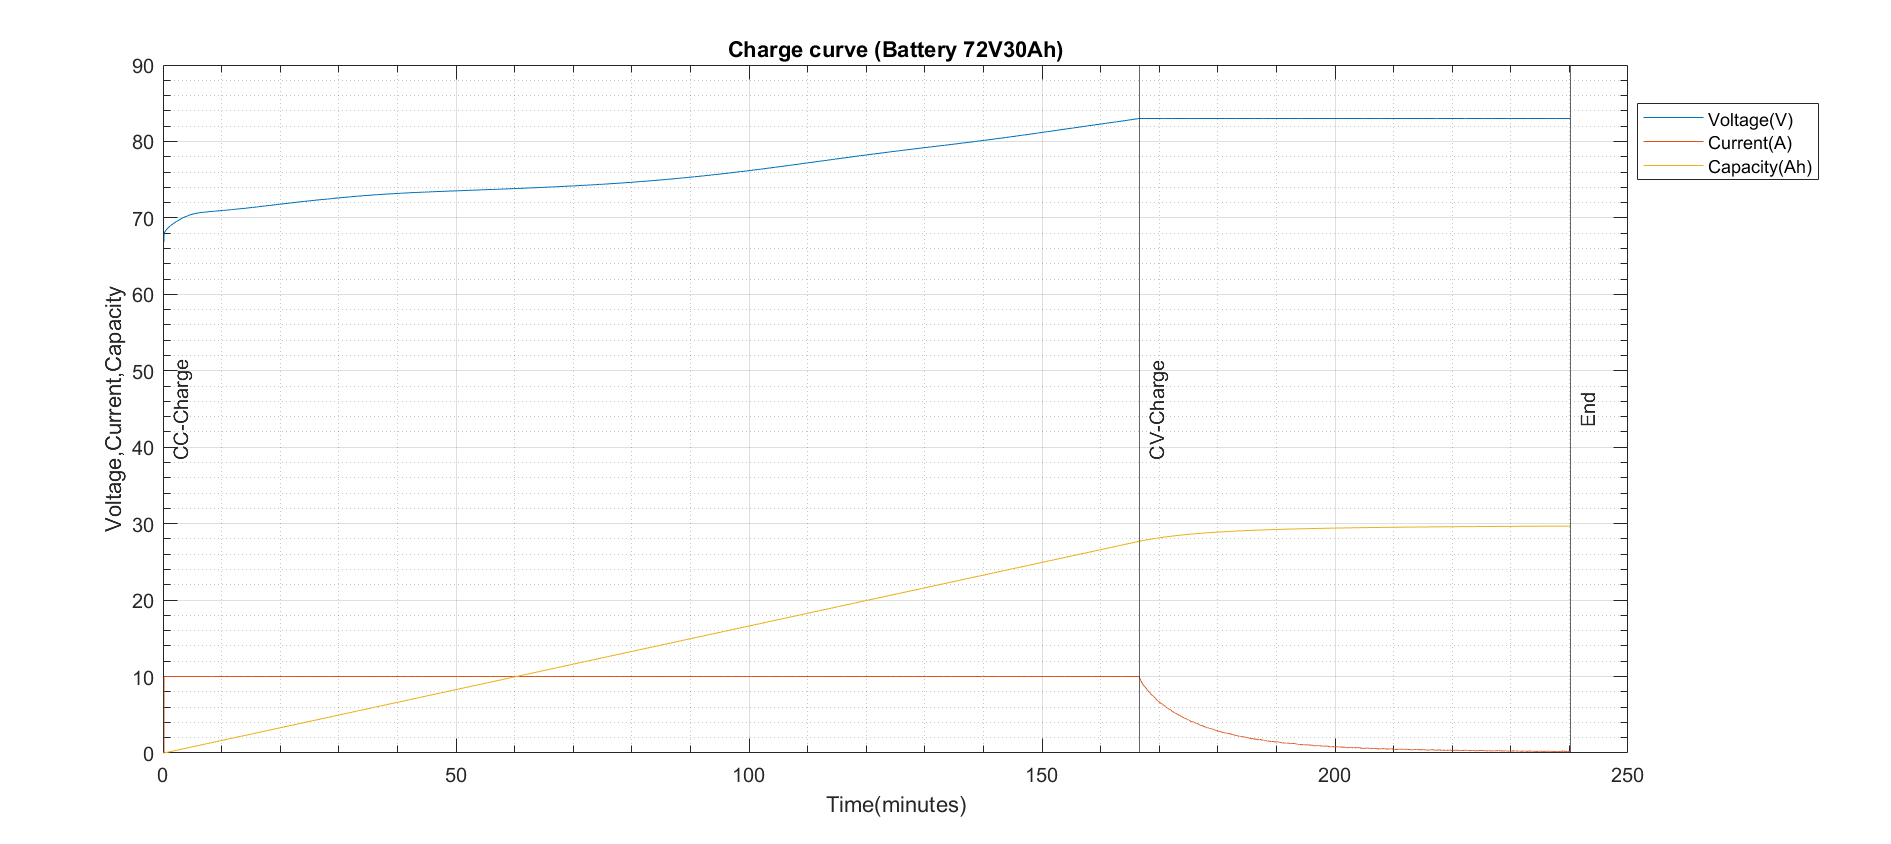
\includegraphics[width=\paperwidth]{Chapters/img/Result/Charge curve 72V30Ah.png}}
		\centering
		\captionsetup{justification=centering,margin=2cm}
		\caption{กราฟการทดสอบการป้องกันการชาร์จเกินของแบตเตอรี่ 72V30Ah}
	\end{figure}
\end{center}
จากการทดสอบพบว่าแบตเตอรี่สำหรับจักรยานยนต์ไฟฟ้าในระหว่างการทดสอบไม่มีการรั่วไหลของอิเล็กโทรไลต์ ไม่มีการแตกหักหรือฉีกขาด ไม่เกิดเพลิงใหม้ และไม่เกิดการระเบิด
โดยการทดสอบการชาร์จนี้ถูกขัดจังหวะโดยระบบการจัดการแบตเตอรี่(BMS)ของโมดูลแบตเตอรี่นี้เองซึ่งเมื่อแบตเตอรี่มีแรงดันเกินกว่าที่ระบบการจัดการแบตเตอรี่กำหนด
หลังจากที่หยุดการชาร์จจากนั้นผู้ทดสอบได้ทำการสังเกตแบตเตอรี่เป็นระยะเวลา 1 ชั่วโมงพบว่าแบตเตอรี่ยังคงสภาพปกติและยังคงสามารถใช้งานได้
\newline
ผลจากการทดสอบแบตเตอรี่สำหรับรถสามล้อไฟฟ้า 72V 60Ah มีดังนี้
\begin{center}
	\begin{figure}[H]
	\makebox[\textwidth]{
	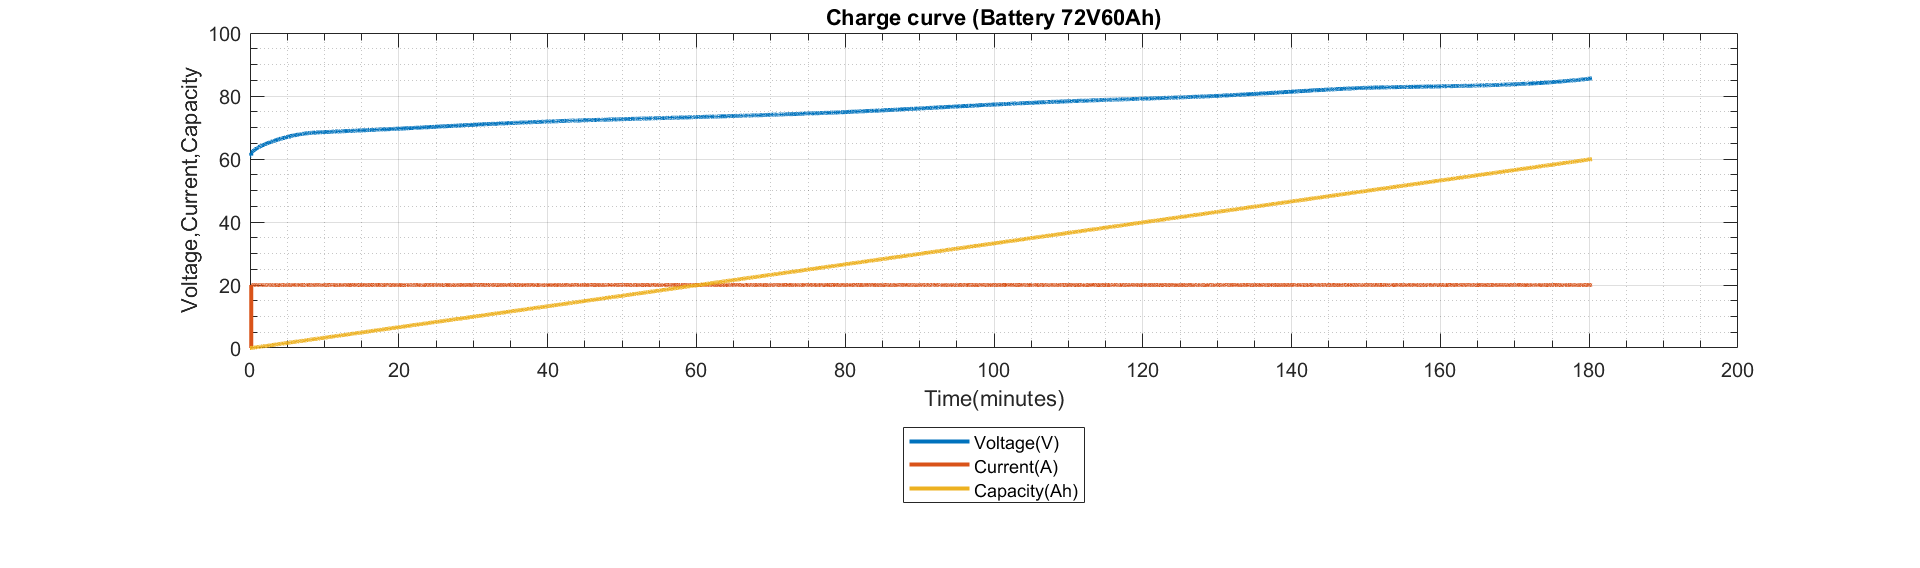
\includegraphics[width=\paperwidth]{Chapters/img/Result/Charge curve 72V60Ah.png}}
		\centering
		\captionsetup{justification=centering,margin=2cm}
		\caption{กราฟการทดสอบการป้องกันการชาร์จเกินของแบตเตอรี่ 72V60Ah}
	\end{figure}
\end{center}
จากการทดสอบพบว่าแบตเตอรี่สำหรับรถสามล้อไฟฟ้าระหว่างการทดสอบไม่มีการรั่วไหลของอิเล็กโทรไลต์ ไม่มีการแตกหักหรือฉีกขาด ไม่เกิดเพลิงใหม้ และไม่เกิดการระเบิด
แต่การทดสอบนั้นถูกขัดจังหวะโดยผู้ทดสอบเองเนื่องจากหากดำเนินการทดสอบต่อไปอาจจะทำให้เกิดความเสียหายกับแบตเตอรี่และอุปกรณ์การทดสอบได้ซึ่ง
หลังจากที่หยุดการชาร์จผู้ทดสอบได้ทำการสังเกตแบตเตอรี่เป็นระยะเวลา 1 ชั่วโมงพบว่าแบตเตอรี่ยังคงสภาพปกติและยังคงสามารถใช้งานได้
\newline
ผลจากการทดสอบแบตเตอรี่ 72V 70Ah มีดังนี้
\begin{center}
	\begin{figure}[H]
	\makebox[\textwidth]{
	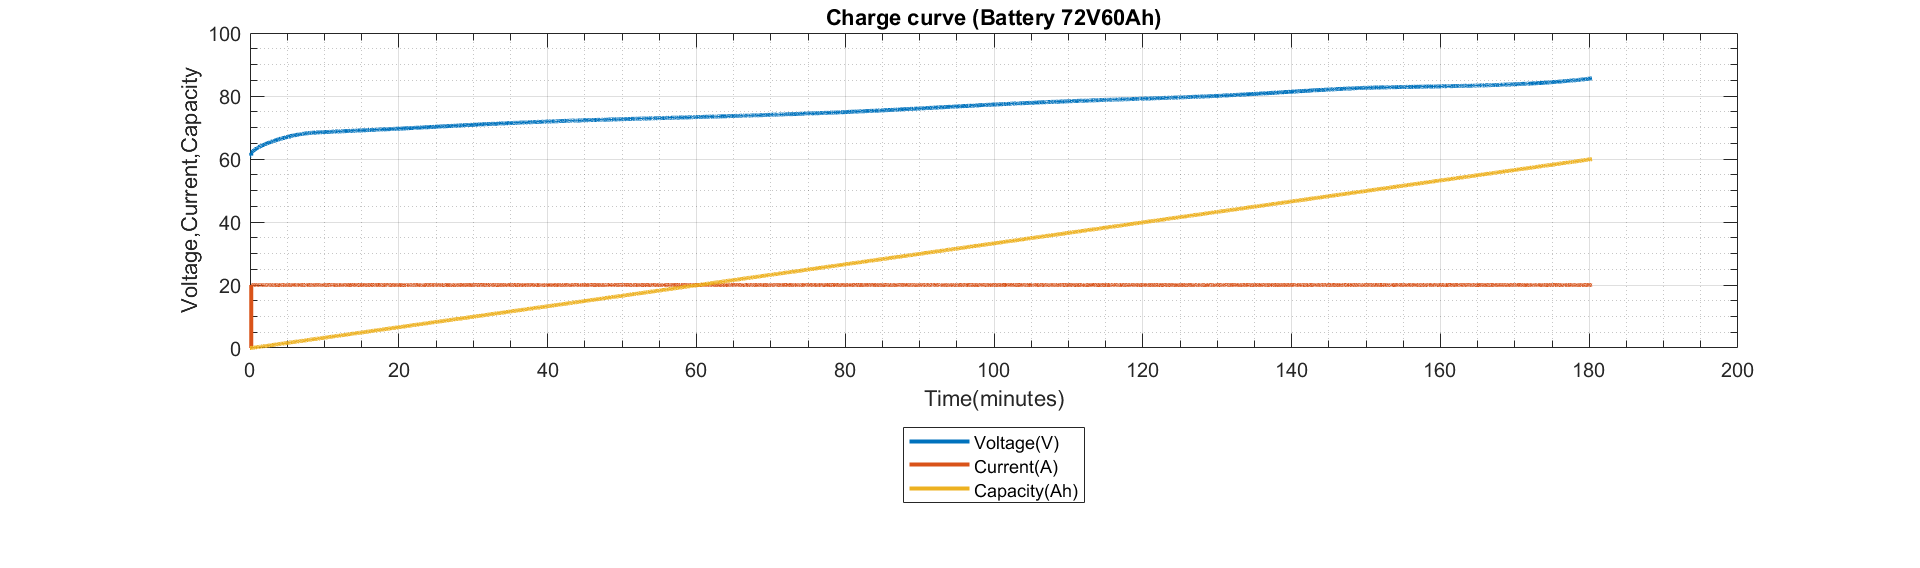
\includegraphics[width=\paperwidth]{Chapters/img/Result/Charge curve 72V60Ah.png}}
		\centering
		\captionsetup{justification=centering,margin=2cm}
		\caption{กราฟการทดสอบการป้องกันการชาร์จเกินของแบตเตอรี่ 72V60Ah}
	\end{figure}
\end{center}
จากการทดสอบพบว่าแบตเตอรี่สำหรับรถสามล้อไฟฟ้าระหว่างการทดสอบไม่มีการรั่วไหลของอิเล็กโทรไลต์ ไม่มีการแตกหักหรือฉีกขาด ไม่เกิดเพลิงใหม้ และไม่เกิดการระเบิด
แต่การทดสอบนั้นถูกขัดจังหวะโดยผู้ทดสอบเองเนื่องจากหากดำเนินการทดสอบต่อไปอาจจะทำให้เกิดความเสียหายกับแบตเตอรี่และอุปกรณ์การทดสอบได้ซึ่ง
หลังจากที่หยุดการชาร์จผู้ทดสอบได้ทำการสังเกตแบตเตอรี่เป็นระยะเวลา 1 ชั่วโมงพบว่าแบตเตอรี่ยังคงสภาพปกติและยังคงสามารถใช้งานได้
%----------------------------------------------------------------------------------
\subsection{ผลการทดสอบการป้องกันการดิสชาร์จเกิน}
สำหรับการทดสอบการป้องกันการดิสชาร์จเกินของแบตเตอรี่สำหรับจักรยานยนต์ไฟฟ้า 72V 30Ah มีดังนี้
\begin{center}
	\begin{figure}[H]
	\makebox[\textwidth]{
	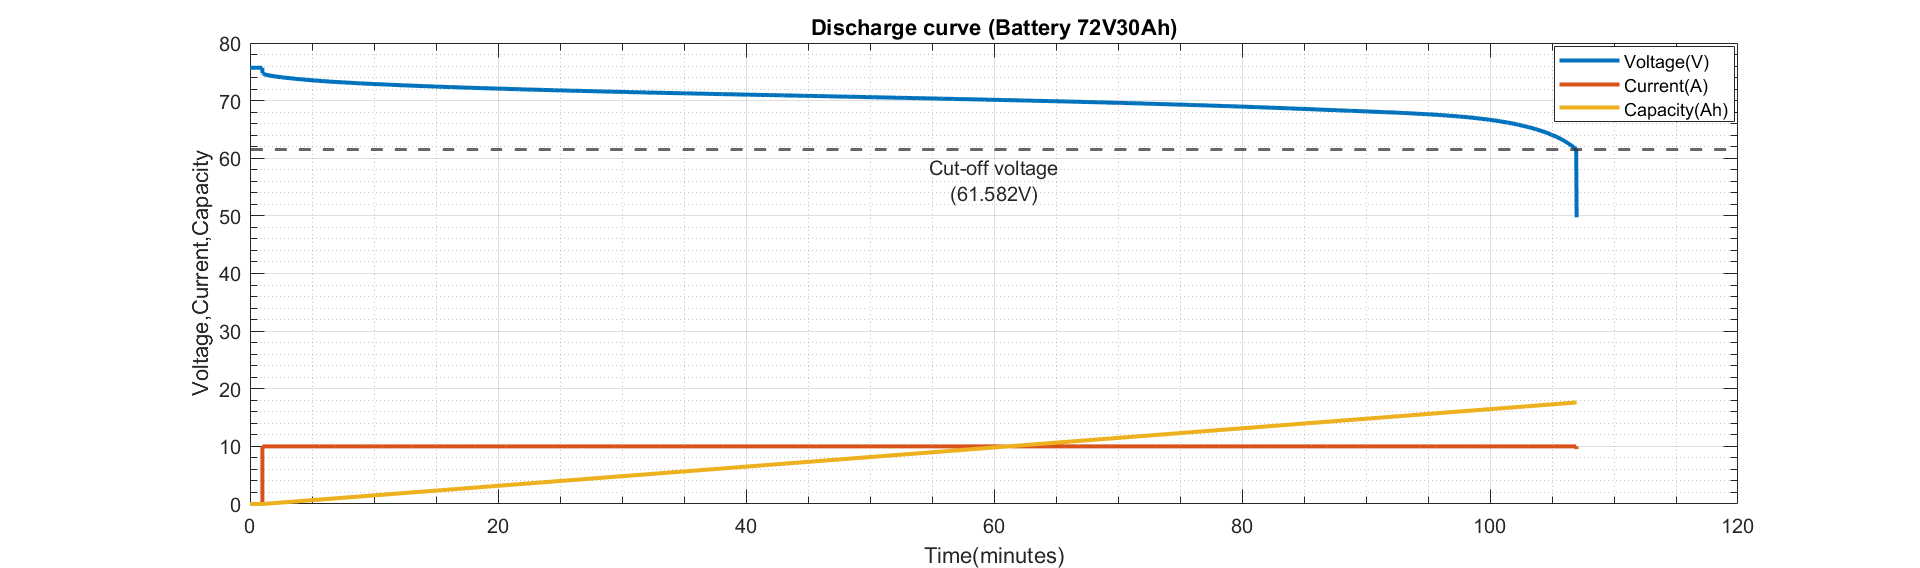
\includegraphics[width=\paperwidth]{Chapters/img/Result/Discharge curve 72V30Ah.png}}
		\centering
		\captionsetup{justification=centering,margin=2cm}
		\caption{กราฟการทดสอบการป้องกันการดิสชาร์จเกินของแบตเตอรี่ 72V30Ah}
	\end{figure}
\end{center}
จากการทดสอบพบว่าแบตเตอรี่สำหรับจักรยานยนต์ไฟฟ้าในระหว่างการทดสอบไม่มีการรั่วไหลของอิเล็กโทรไลต์ ไม่มีการแตกหักหรือฉีกขาด ไม่เกิดเพลิงใหม้ และไม่เกิดการระเบิด
โดยการทดสอบการดิสชาร์จนี้ถูกขัดจังหวะโดยระบบการจัดการแบตเตอรี่(BMS)ของโมดูลแบตเตอรี่นี้เองซึ่งเมื่อแบตเตอรี่มีแรงดันต่ำเกินกว่าที่ระบบการจัดการแบตเตอรี่กำหนด
หลังจากที่หยุดการดิสชาร์จจากนั้นผู้ทดสอบได้ทำการสังเกตแบตเตอรี่เป็นระยะเวลา 1 ชั่วโมงพบว่าแบตเตอรี่ยังคงสภาพปกติและยังคงสามารถใช้งานได้
\newline
ผลจากการทดสอบแบตเตอรี่สำหรับรถสามล้อไฟฟ้า 72V 60Ah มีดังนี้
\begin{center}
	\begin{figure}[H]
	\makebox[\textwidth]{
	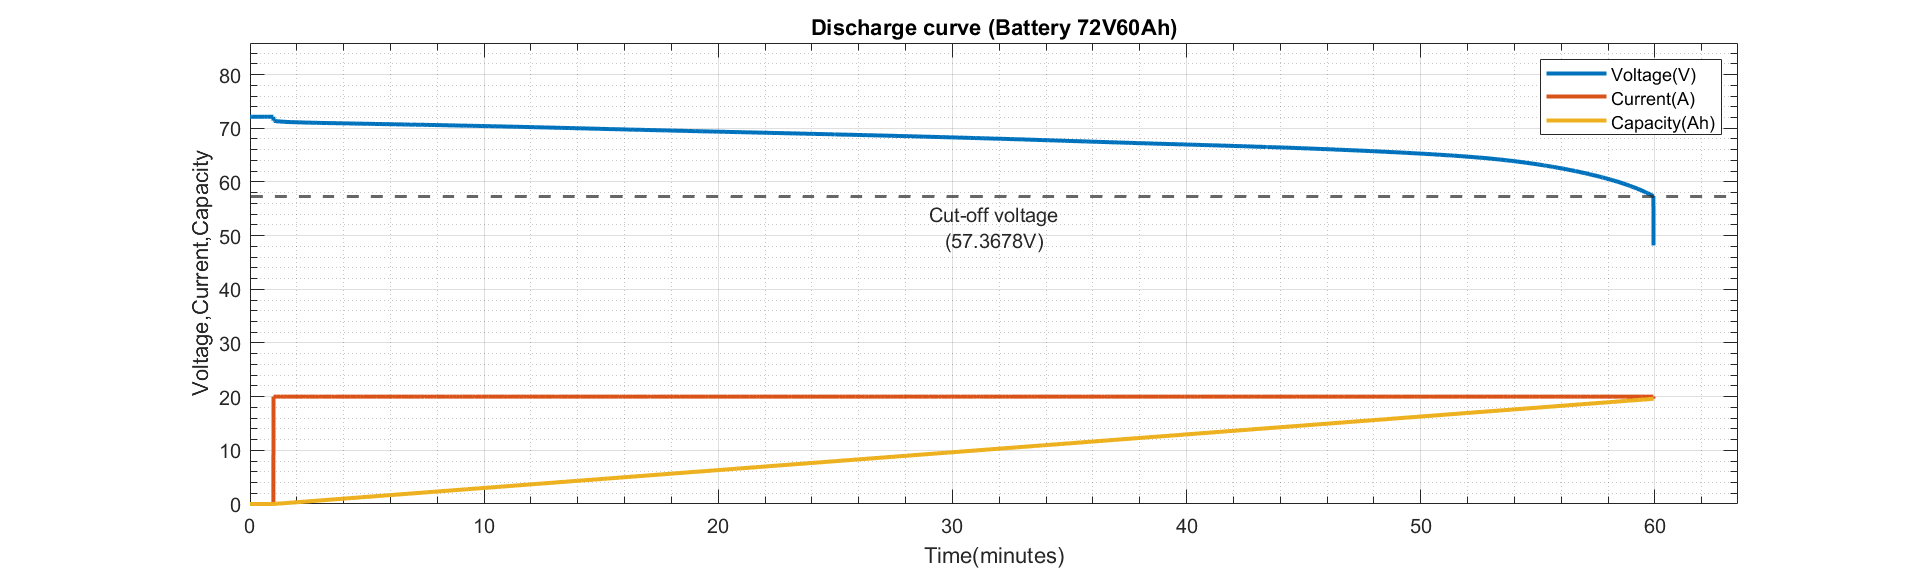
\includegraphics[width=\paperwidth]{Chapters/img/Result/Discharge curve 72V60Ah.png}}
		\centering
		\captionsetup{justification=centering,margin=2cm}
		\caption{กราฟการทดสอบการป้องกันการดิสชาร์จเกินของแบตเตอรี่ 72V60Ah}
	\end{figure}
\end{center}
จากการทดสอบพบว่าแบตเตอรี่สำหรับรถสามล้อไฟฟ้าระหว่างการทดสอบไม่มีการรั่วไหลของอิเล็กโทรไลต์ ไม่มีการแตกหักหรือฉีกขาด ไม่เกิดเพลิงใหม้ และไม่เกิดการระเบิด
โดยการทดสอบการดิสชาร์จนี้ถูกขัดจังหวะโดยระบบการจัดการแบตเตอรี่(BMS)ของโมดูลแบตเตอรี่นี้เองซึ่งเมื่อแบตเตอรี่มีแรงดันต่ำเกินกว่าที่ระบบการจัดการแบตเตอรี่กำหนด
หลังจากที่หยุดการดิสชาร์จจากนั้นผู้ทดสอบได้ทำการสังเกตแบตเตอรี่เป็นระยะเวลา 1 ชั่วโมงพบว่าแบตเตอรี่ยังคงสภาพปกติและยังคงสามารถใช้งานได้









